\documentclass[compress,]{beamer}

%presentation layout

\mode<presentation>
{
  \usetheme{Berlin}
  % \usecolortheme{dove}
  \setbeamercolor{structure}{bg=black,fg=white}
  \setbeamercolor{normal text}{bg=black,fg=white}
  \setbeamercolor{titlepage}{bg=black,fg=white}
  \setbeamercolor{titlelike}{bg=black,fg=white}
  \setbeamercolor{palette primary}{bg=black}
  \setbeamercolor{palette secondary}{bg=black, fg=gray}
  \setbeamercolor{palette tertiary}{bg=black, fg=gray}
  \setbeamercolor{palette quarternary}{bg=black}
  \setbeamercovered{transparent}
  \useinnertheme{rectangles}
  %\usefonttheme{serif}
}

\setbeamertemplate{navigation symbols}{}

%loading packages
\usepackage[ngerman]{babel}
\usepackage[T1]{fontenc}
\usepackage[utf8]{inputenc}
\usepackage{graphicx}
\usepackage{amsmath}
\usepackage{framed}

% vorgeplaenkel
\title[StAPf-Bericht]{StAPF-Bericht}

\author{Ständiger Ausschuss aller Physikfachschaften}

\institute[Zusammenkunft aller Physikfachschaften]

\date{19. November 2015}

\subject{ZäPFchen-Einführung}

\begin{document}

\begin{frame}[plain]{}
  \titlepage

   \begin{figure}
     \centering
     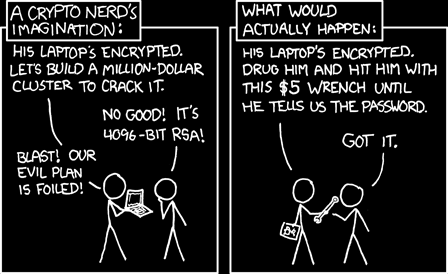
\includegraphics[width=0.6\textwidth]{security_inverted.png}
	 \\ \hspace{3cm} {\tiny source: https://xkcd.com/538/}
   \end{figure}
\end{frame}

\section{Zusammensetzung}

\begin{frame}{Aktuelle Zusammensetzung}
	\begin{itemize}
		\item Adriana Röttger (Münster)
		\item Björn Guth (Aachen)
		\item Jakob Schnell (Heidelberg)
		\item \emph{Lea Meyer} (Kiel)
		\item \emph{Niklas Luhmann} (Konstanz)
	\end{itemize}
	\textbf{In einer Nebenrolle:} TOPF
	\begin{itemize}
		\item Fabian Freyer
		\item Jörg Behrmann
	\end{itemize}
\end{frame}

\begin{frame}{Öffentlichkeitsarbeit}
	\begin{itemize}
		\item Resolutionen veröffentlicht
			\begin{itemize}
				\item Koordination mit KoMa beidseitig langwierig
				\item Reaktion auf Übungskonzepte:
					\begin{itemize}
						\item verpflichtende Übungen?
						\item Übungsleistung als Teil der Modulleistung?
					\end{itemize}
			\end{itemize}
		\item Bericht verschickt
	\end{itemize}
\end{frame}

\section{Akkreditierung}

\begin{frame}{Akkreditierungspool}
	\begin{itemize}
		\item 19 Personen im \emph{Progammakkreditierungspool}\\
			6 Personen im \emph{Systemakkredierungspool}
			\begin{itemize}
				\item[$\rightarrow$] Auslaufende Mandate: Thomas Rudzki (Heidelberg)
			\end{itemize}
		\item PVT ??
		\item kommendes PVT im Dezember abgesagt
		\item nächstes PVT 8. bis 10. April 2016 (Ort wird noch gesucht)
	\end{itemize}
\end{frame}

\begin{frame}
	\begin{framed}
		\begin{center}
			{\Huge \textbf{Wichtig}}\\
			\vspace{0.5cm}
			{\Large Aktuelle Anmeldeformulare für den Pool ausfüllen und in digitaler Form an die Verwaltung senden}
		\end{center}
	\end{framed}
\end{frame}

\section{MeTaFa}

\begin{frame}{MeTaFa}
	\begin{itemize}
		\item Treffen in Braunschweig (25. bis 27. November 2015)
			\begin{itemize}
				\item[$\rightarrow$] Themen: Ist-Zustand BuFatas, Veröffentlichungwege, Flüchtlinge
			\end{itemize}
		\item Nächstes Treffen scheint noch nicht festzustehen
	\end{itemize}
\end{frame}

\section{KommGrem}

\begin{frame}{KommGrem}
	\begin{itemize}
		\item[] ZaPF:
			\begin{itemize}
				\item Thomas Rudzki (Heidelberg)
				\item Zafer El-Mokdad (Potsdam)
			\end{itemize}
		\item[] jDPG:
			\begin{itemize}
				\item Eric Abraham (Jena)
				\item Hejo Kerl (Zürich)
			\end{itemize}
	\end{itemize}
	\vspace{0.5cm}
	\textbf{Sprecher}: Eric Abraham
\end{frame}
\end{document}
